% Options for packages loaded elsewhere
\PassOptionsToPackage{unicode}{hyperref}
\PassOptionsToPackage{hyphens}{url}
%
\documentclass[
  12pt,
]{article}
\usepackage{lmodern}
\usepackage{amsmath}
\usepackage{ifxetex,ifluatex}
\ifnum 0\ifxetex 1\fi\ifluatex 1\fi=0 % if pdftex
  \usepackage[T1]{fontenc}
  \usepackage[utf8]{inputenc}
  \usepackage{textcomp} % provide euro and other symbols
  \usepackage{amssymb}
\else % if luatex or xetex
  \usepackage{unicode-math}
  \defaultfontfeatures{Scale=MatchLowercase}
  \defaultfontfeatures[\rmfamily]{Ligatures=TeX,Scale=1}
\fi
% Use upquote if available, for straight quotes in verbatim environments
\IfFileExists{upquote.sty}{\usepackage{upquote}}{}
\IfFileExists{microtype.sty}{% use microtype if available
  \usepackage[]{microtype}
  \UseMicrotypeSet[protrusion]{basicmath} % disable protrusion for tt fonts
}{}
\makeatletter
\@ifundefined{KOMAClassName}{% if non-KOMA class
  \IfFileExists{parskip.sty}{%
    \usepackage{parskip}
  }{% else
    \setlength{\parindent}{0pt}
    \setlength{\parskip}{6pt plus 2pt minus 1pt}}
}{% if KOMA class
  \KOMAoptions{parskip=half}}
\makeatother
\usepackage{xcolor}
\IfFileExists{xurl.sty}{\usepackage{xurl}}{} % add URL line breaks if available
\IfFileExists{bookmark.sty}{\usepackage{bookmark}}{\usepackage{hyperref}}
\hypersetup{
  hidelinks,
  pdfcreator={LaTeX via pandoc}}
\urlstyle{same} % disable monospaced font for URLs
\usepackage[margin=1in]{geometry}
\usepackage{graphicx}
\makeatletter
\def\maxwidth{\ifdim\Gin@nat@width>\linewidth\linewidth\else\Gin@nat@width\fi}
\def\maxheight{\ifdim\Gin@nat@height>\textheight\textheight\else\Gin@nat@height\fi}
\makeatother
% Scale images if necessary, so that they will not overflow the page
% margins by default, and it is still possible to overwrite the defaults
% using explicit options in \includegraphics[width, height, ...]{}
\setkeys{Gin}{width=\maxwidth,height=\maxheight,keepaspectratio}
% Set default figure placement to htbp
\makeatletter
\def\fps@figure{htbp}
\makeatother
\setlength{\emergencystretch}{3em} % prevent overfull lines
\providecommand{\tightlist}{%
  \setlength{\itemsep}{0pt}\setlength{\parskip}{0pt}}
\setcounter{secnumdepth}{-\maxdimen} % remove section numbering
\usepackage{setspace}\doublespacing
\usepackage{amsmath}
\usepackage{lineno}
\linenumbers
\usepackage{fontspec}
\setmainfont{Times New Roman}
\usepackage{booktabs}
\usepackage{booktabs}
\usepackage{longtable}
\usepackage{array}
\usepackage{multirow}
\usepackage{wrapfig}
\usepackage{float}
\usepackage{colortbl}
\usepackage{pdflscape}
\usepackage{tabu}
\usepackage{threeparttable}
\usepackage{threeparttablex}
\usepackage[normalem]{ulem}
\usepackage{makecell}
\usepackage{xcolor}
\ifluatex
  \usepackage{selnolig}  % disable illegal ligatures
\fi
\newlength{\cslhangindent}
\setlength{\cslhangindent}{1.5em}
\newlength{\csllabelwidth}
\setlength{\csllabelwidth}{3em}
\newenvironment{CSLReferences}[2] % #1 hanging-ident, #2 entry spacing
 {% don't indent paragraphs
  \setlength{\parindent}{0pt}
  % turn on hanging indent if param 1 is 1
  \ifodd #1 \everypar{\setlength{\hangindent}{\cslhangindent}}\ignorespaces\fi
  % set entry spacing
  \ifnum #2 > 0
  \setlength{\parskip}{#2\baselineskip}
  \fi
 }%
 {}
\usepackage{calc}
\newcommand{\CSLBlock}[1]{#1\hfill\break}
\newcommand{\CSLLeftMargin}[1]{\parbox[t]{\csllabelwidth}{#1}}
\newcommand{\CSLRightInline}[1]{\parbox[t]{\linewidth - \csllabelwidth}{#1}\break}
\newcommand{\CSLIndent}[1]{\hspace{\cslhangindent}#1}

\author{}
\date{\vspace{-2.5em}}

\begin{document}

\textbf{Choosing priors in Bayesian ecological models by simulating from
the prior predictive distribution}

Jeff S. Wesner and Justin P.F. Pomeranz

University of South Dakota, Department of Biology, Vermillion, SD 57069

\href{mailto:Jeff.Wesner@usd.edu}{\nolinkurl{Jeff.Wesner@usd.edu}}

\newpage

\textbf{Abstract}

Bayesian data analysis is increasingly used in ecology, but prior
specification remains focused on choosing non-informative priors (e.g.,
flat or vague priors). One barrier to choosing more informative priors
is that priors must be specified on model parameters (e.g., intercepts,
slopes, sigmas), but prior knowledge often exists on the level of the
response variable. This is particularly true for common models in
ecology, like generalized linear mixed models that have a link function
and potentially dozens of parameters, each of which needs a prior
distribution. We suggest that this difficulty can be overcome by
simulating from the prior predictive distribution and visualizing the
results on the scale of the response variable. In doing so, some common
choices for non-informative priors on parameters can easily be seen to
produce biologically impossible values of response variables. Such
implications of prior choices are difficult to foresee without
visualization. We demonstrate a workflow for prior selection using
simulation and visualization with two ecological examples (predator-prey
body sizes and spider responses to food competition). This approach is
not new, but its adoption by ecologists will help to better incorporate
prior information in ecological models, thereby maximizing one of the
benefits of Bayesian data analysis.

Keywords: \emph{Bayesian, prior predictive distribution, GLMM,
simulation}

\newpage

\textbf{Introduction}

The distinguishing feature between Bayesian and non-Bayesian statistics
is that Bayesian statistics treats unknown parameters as random
variables governed by a probability distribution, while non-Bayesian
statistics treats unknown parameters as fixed and unknown quantities
(Ellison 2004, Hobbs and Hooten 2015). A common misconception is that
only Bayesian statistics incorporates prior information. However,
non-Bayesian methods can and often do incorporate prior information,
either informally in the choices of likelihoods and model structures, or
formally as penalized likelihood or hierarchical modeling (Hobbs and
Hooten 2015, Morris et al. 2015).

While prior information is not unique to Bayesian models, it is required
of them. For example, in a simple linear regression of the form
\(y \sim \text{Normal}(\upalpha + \beta x, \sigma)\), the intercept
\(\alpha\), slope \(\beta\), and standard deviation \(\sigma\) are
unknown parameters that each need a prior probability distribution.
There are differing opinions and philosophies on the best practices for
choosing priors (Lindley 1961, Edwards et al. 1963, Morris et al. 2015,
Wolf et al. 2017, Gelman et al. 2017, Lemoine 2019, Banner et al. 2020).
In ecology, a common practice is to assign so-called non-informative
priors that effectively assign equal probability to all possible values
using either uniform or diffuse normal priors with large variances
(Lemoine 2019). These priors allow Bayesian inference to proceed (i.e.,
produce a posterior distribution), but with presumably limited influence
of the priors (Lemoine 2019).

Reasons for using non-informative priors are varied but are at least in
part driven by a desire to avoid the appearance of subjectivity and/or a
reliance on default settings in popular software (Gelman and Hennig
2017, Banner et al. 2020). There are several arguments against this
approach. First, ``non-informative'' is a misnomer. All proper priors
influence the posterior distribution to some extent (Hobbs and Hooten
2015). As a result, a prior cannot just be assumed as non-informative
based on default settings or a wide variance (Seaman III et al. 2012).
Its implications for the model should be checked just like any other
subjective assumption in data analysis, whether Bayesian or not (Gelman
et al. 2017, Banner et al. 2020). Second, adhering to non-informative
priors removes a major potential benefit of Bayesian analysis, which is
to explicitly incorporate prior research and expertise into new science
(Hobbs and Hooten 2015, Lemoine 2019, Rodhouse et al. 2019). Third,
informative priors can help to reduce spurious conclusions due to errors
in magnitude or sign of a relationship by treating extreme values in the
data skeptically (Gelman et al. 2012, Lemoine 2019). Finally,
informative priors make computational algorithms like MCMC run more
efficiently, which can save hours or days of computing time in complex
models (Hobbs and Hooten 2015). An additional way to improve efficiency
can come from different choices of prior distributions, such as an
inverse-gamma distribution on the variance rather than the exponential
prior on the standard deviation that we use in the models here, for
example. For more complete discussion on this, see Gelman and others
(2006).

While there are clear arguments for why ecologists \emph{should} use
more informative priors, it is often difficult to know \emph{how} to use
them. Even for seemingly simple and routine models, like logistic or
Poisson regression, it can be difficult to understand \emph{a priori}
how priors affect the model, because they must be assigned in the
context of likelihood with a linearizing link-function (Seaman III et
al. 2012, Gelman et al. 2017). In other words, prior specification takes
place on model parameters (e.g., slopes, intercepts, variances), but
prior knowledge is often easier to assess on the model outcomes (Kadane
et al. 1980, Bedrick et al. 1996, Gabry et al. 2019). This is
particularly true for models that are commonly used in ecology, such as
generalized linear mixed models with interactions. These models may have
dozens of parameters and hyperparameters, each of which require a prior
probability distribution (Bedrick et al. 1996, McElreath 2020).

We suggest that ecologists can address this problem by simulating from
the prior predictive distribution and visualizing the implications of
the priors on outcomes of interest (e.g., means and confidence intervals
of treatment groups, simulated data, or regression lines). In this
paper, we demonstrate this approach using two case studies with
ecological data (Figure 1). All data and code are available at:
\url{https://github.com/jswesner/prior_predictive}.

\textbf{Prior Predictive Simulation}

An attractive feature of the Bayesian approach is that the models are
generative. This means that we can simulate potential data from the
model so long as the parameters are assigned a proper probability
distribution (Gelman et al. 2013). This feature is routinely used to
check models and prior influence \emph{after} fitting the data using the
posterior predictive distribution (Lemoine 2019, Gelman et al. 2020),
but it can also be used before seeing the data using the prior
predictive distribution (Gabry et al. 2019).

The general workflow for prior predictive simulation is:

\begin{enumerate}
\def\labelenumi{\arabic{enumi})}
\item
  Draw N realizations from a prior distribution
\item
  For each draw, simulate a model outcome or new data from the
  likelihood
\item
  Plot the results
\item
  Use domain knowledge to assess whether simulated values reflect prior
  knowledge
\item
  If simulated values do not reflect prior knowledge, change the prior
  distribution, likelihood, or both and repeat the simulation from step
  1
\item
  If simulated values reflect prior knowledge, add the data and estimate
  the posterior distribution
\end{enumerate}

This amounts to a prior predictive check to satisfy the expectation that
``simulations from the full Bayesian model\ldots should be plausible
data sets'' (Kennedy et al. 2019). We demonstrate it with two motivating
examples.

\textbf{Example 1: Predator-Prey Body Sizes - Simple Linear Regression}

\emph{Data} - Understanding predator-prey interactions has long been a
research interest of ecologists. Body size is related to a number of
aspects that influence these interactions. For example, predators are
often gape-limited, meaning that larger predators should be able to eat
larger prey. The data set of Brose et al. (2006) documents 13,085
predator-prey interactions, including the mean mass of each (Figure 1a).

\emph{Model} - We examined the hypothesis that the prey body mass
increases log-linearly with predator body mass using a simple linear
model:

\textbackslash begin\{align\} \textbackslash text\{log\} (y\_i)
\textbackslash sim \textbackslash text\{Normal\}(\textbackslash mu\_i,
\textbackslash sigma)\textbackslash\textbackslash{} \textbackslash mu\_i
= \textbackslash alpha + \textbackslash beta
\textbackslash text\{log\}(x\_i)\textbackslash\textbackslash{}
\textbackslash alpha \textbackslash sim \textbackslash text\{Normal\}(0,
\textbackslash sigma\_\{\textbackslash alpha\})\textbackslash\textbackslash{}
\textbackslash beta \textbackslash sim \textbackslash text\{Normal\}(0,
\textbackslash sigma\_\{\textbackslash beta\})\textbackslash\textbackslash{}
\textbackslash sigma \textbackslash sim
\textbackslash text\{Exponential\}(\textbackslash phi)
\textbackslash end\{align\} where \(\text{log}(y_i)\) is natural log
transformed prey mass and \(\text{log}(x_i)\) is natural log transformed
predator mass.

\emph{Priors} - For the \(\alpha\) and \(\beta\) priors, we first assign
a mean of 0 with a ``non-informative'' standard deviation of 1000
{[}\(N(0, 1000)\){]} (Table 1). These prior values are often used as
defaults, especially in earlier Bayesian software to generate ``flat''
prior distributions and are commonly used in the ecological literature
(McCarthy and Masters 2005, Banner et al. 2020). The mean of 0 in a
normal distribution implies that the intercept and slope have equal
probability of being positive or negative. For the exponential
distribution, we specify an initial \(\phi\) of 0.00001, chosen by
plotting 100 simulations from the exponential function in R (R Core Team
2020) with varying values of \(\phi\) {[}e.g.,
\texttt{plot(rexp(100,\ 0.00001)}{]}. A value of 0.00001 generated an
average deviance of \textasciitilde1,000 with values up to
\textasciitilde5,000, indicating the possibility of producing extremely
large values.

After simulating regressions from these initial priors, we specified
successfully tighter priors and repeated the simulations (Table 1;
Figure 2). Those simulations were compared to reference points
representing prior knowledge (Mass of earth, a Blue Whale, a virus, and
a Carbon-12 atom). The goal was to use these reference points to find a
joint prior distribution that produced reasonable values of potential
prey masses. We did this using two levels of the model (\(\mu_i\) and
\(y_i\)). For \(\mu_i\), we simulated 100 means across each value of
\(x_i\) and plotted them as regression lines. For \(y_i\), we simulated
a fake data set containing simulated values of log prey mass for each of
the 13,085 values of log predator mass (\(x_i\)) in the Brose et al.
(2006) data.

\emph{Results} - The weak ``non-informative'' priors make nonsense
predictions (Figure 2a-c). In Figure 2a, all of the lines are impossibly
steep, suggesting that predators could plausibly eat prey that are
larger than earth or smaller than an atom. The stronger priors in Figure
2b suffer from the same problem, though the effect is less severe. The
strongest priors (Figure 2c) produce more reasonable predictions, though
they are still quite vague, with positive probability that predators
could eat prey larger than an adult Blue Whale. The simulated fake data
sets tell a similar story (Figure 2d-f), but with the added influence of
\(\sigma\) (Equation 1).

We fit the model using the strongest prior set and overlaid these on the
prior simulations (Figure 2c,f). As expected, there is a strong positive
relationship between log predator and log prey size (Figure 2c - orange
line), despite the uncertainty in the prior. The intercept is -4.8 ±
0.04 (mean ± sd), indicating that a predator weighing 1 gram (wet or dry
mass) would eat prey 2-3 orders of magnitude smaller than the predator.
The slope is 0.6 ± 0.01, indicating a reliably positive relationship
such that an increase in 1 log unit of predator mass corresponds with an
increase in prey mass of 0.6 log units on average. Sigma is 3.7 ± 0.02,
indicating an average residual for individual predator-prey data or +/-
3.7 log-units of prey mass. This is reflected in the simulated data,
which show a wide range of simulated predator-prey size pairings, but
all are within a reasonable range compared to prior predictions (Figure
2f).

There are several benefits to choosing a stronger prior. First, it is
difficult to justify the two weakest priors on biological grounds. They
place large amounts of prior probability on impossible values. This can
matter when priors need to be justified to a granting agency or to
reviewers. More critically, specification of priors can have
conservation or legal implications, and the ability to justify priors
with simulation helps to improve transparency (Crome et al. 1996, Banner
et al. 2020). Stronger priors also improve computational efficiency
(McElreath 2020). We fit these models using the \emph{brms} package
(Burkner 2017). The algorithms associated with models that had the
stronger or strongest priors were up to 50\% faster than the model with
weak priors, taking 56 vs 28 seconds on a standard laptop (compilation
time + warmup time + sampling time). For more complex models with
algorithms that take longer to run, this improvement can save hours or
days of computing time.

\emph{Caveats} - We know from the literature that predators are
generally larger than their prey by 2-3 orders of magnitude (Trebilco et
al. 2013). Therefore, it would make sense to alter the prior mean of the
intercept to a value below zero, perhaps using an average predator/prey
mass comparison from the literature. That is apparent from the prior
versus posterior comparison in Figure 2c. Similarly, the fact that
larger predators tend to eat larger prey is well-known, so the prior on
the slope \(\beta\) could be changed to a positive mean. Another option
is to standardize the predictor variable(s)
(\(x_{standardized} = \frac{x-\bar{x}}{\sigma_{x}}\)) so that the
regression slopes can be interpreted as units of standard deviation.
This also improves interpretation of the intercept when values of zero
(e.g., prey mass = 0) do not make sense (McElreath 2020). This would be
most relevant in the current model if prey mass was included as raw
mass, rather than log mass.

\textbf{Example 2: Spider Abundance - Generalized Linear Mixed Model}

\emph{Data} - This data set comes from Warmbold and Wesner (2018), who
measured terrestrial spider responses to different combinations of
freshwater fish using fish enclosure cages in a backwater of the
Missouri River, USA. They hypothesized that fish would reduce the
emergence of adult aquatic insects by eating the larvae of those insects
in the water, causing a reduction in terrestrial spiders that feed on
the adult forms of those insects. The original experiment contained six
treatments. We present a simplified version comparing spider abundance
above three treatments that contain either Smallmouth Buffalo
(\emph{Ictiobus bubalus}), Green Sunfish (\emph{Lepomis cyanellus}), or
a fishless control. Each treatment had four replicates for a total of 12
cages (each 2.3 m\(^2\)). The cages were arranged in two rows, one on
either side of the shoreline of the backwater. The treatments were then
randomly assigned to cages while ensuring that each treatment was
represented at least once in each row. The number of occupied spider
webs above each cage was counted on four dates over the 29-day
experiment (Figure 1b).

\emph{Model} - We fit a generalized linear mixed model with a Poisson
likelihood, since the response variable (\# webs per cage) is a
non-negative integer. The predictor variables were date, treatment, and
a date \(\times\) treatment interaction with a random intercept for
cages. The interaction is included because it was expected that the
effect of fish on spider counts would vary across sampling dates in
response to variation in insect emergence. Date was a categorical
variable with four levels representing four sampling dates. Treatment
was a categorical variable with three levels representing the Smallmouth
Buffalo, Green Sunfish, or fishless control. Describing the model as
having two main effects and an interaction is deceptively simple. In
reality, the model has 13 parameters that require a prior specification:
11 ``fixed'' effects that indicate all combinations of date \(\times\)
treatment, plus 1 intercept and a hyperprior \(\phi\) on the intercept:

\textbackslash begin\{gather\} y\_i \textbackslash sim
\textbackslash text\{Poisson\}(\textbackslash lambda\_i)\textbackslash\textbackslash{}
\textbackslash text\{log\} (\textbackslash lambda\_i) =
\textbackslash alpha + \textbackslash alpha\_\{{[}cage{]}\}
+\textbackslash beta\_1x\_\{trt\_i = fishless\} +
\textbackslash beta\_2x\_\{trt\_i = green\} +
\ldots\textbackslash beta\_\{11\}x\_\{trt\_i = green:date\_i =
4\}\textbackslash\textbackslash{} \textbackslash alpha
\textbackslash sim \textbackslash text\{Normal\}(0,
\textbackslash sigma\_\{\textbackslash alpha\})\textbackslash\textbackslash{}
\textbackslash alpha\_\{{[}cage\_\{1-12\}{]}\} \textbackslash sim
\textbackslash text\{Normal\}(0,
\textbackslash sigma\_\{cage\})\textbackslash\textbackslash{}
\textbackslash beta\_\{1\ldots11\} \textbackslash sim
\textbackslash text\{Normal\}(0,
\textbackslash sigma\_\{\textbackslash beta\_\{1\ldots11\}\})\textbackslash\textbackslash{}
\textbackslash sigma\_\{cage\} \textbackslash sim
\textbackslash text\{Exponential\}(\textbackslash phi)
\textbackslash end\{gather\} where each \(y_i\) is described by a
Poisson distribution with mean \(\lambda_i\). Because the likelihood is
not normal, we specify a log link, \(\text{log}(\lambda_i)\), so that
the mean can be estimated as a linear function of predictors. The
intercept \(\alpha\) represents the predicted log mean number of spiders
in the treatment with Smallmouth Buffalo on the first sample date. The
choice of reference treatment is arbitrary. Choosing Smallmouth Buffalo
and the first date as the intercept is the default choice in R (R Core
Team 2020) because the treatment is coded first alphabetically
(``buffalo'') and first numerically (``2015-06-08'').

The random effect for cage \(\alpha_{cage}\) represents the average
deviation of each cage from the global mean intercept \(\alpha\). It
allows us to account for the fact that individual cages may vary in
their starting densities of spiders (i.e., in their intercepts) for
reasons beyond random sampling. One way in which cages could vary is
their proximity to the shoreline or in their microclimates that cause
variation in wind dispersal of spiders. These unmeasured differences
mean that the cages are not independent and identically distributed,
thus violating the exchangeability assumption. The random effect (i.e.,
varying intercept) allows us to overcome this assumption by allowing
each cage to have its own mean intercept (Hobbs and Hooten 2015).

\emph{Priors} - As before, we simulated outcomes under three model
scenarios, each with different priors (Table 1; Figure 3a-c). Another
complication in this model is the log-link, which changes the biological
interpretation of the parameters. With a Poisson likelihood and
log-link, parameter values must be exponentiated and then interpreted as
a multiplier. Thus, a value of 1.5 for the \(\beta_x\) indicates that
the treatment contains exp(1.5) = 4.5 \emph{times} more spiders than the
reference treatment on the first sample date. This is an example of the
principle that the prior can only be understood in the context of the
likelihood (Gelman et al. 2017).

\emph{Results} - If all we knew was that spiders were counted above 2.32
m\(^2\) cages but we did not know anything else about the experiment
(i.e., the ecosystem, the question, the spider taxa), then we could
still use the prior predictive distribution to select more informative
priors. The weakest priors place substantial probabilities on values of
\textgreater100,000 spiders per cage \emph{on average} (Figure 3a), and
include a small number of predictions on the final sample date with more
than 100 million spiders (Figure 3c). We looked up the range of spider
masses (\textasciitilde0.0005 to 170 grams). If we assume our spiders
are relatively small, say 0.01 grams, then 100 million spiders would
equal 30 tons of spiders. This is approximately equal to the mass of
\textasciitilde6 adult hippopotamus's (each \textasciitilde4 tons).

However, in this case we do have prior information. In a previous study
using the same cages in the same backwater, Warmbold (2016) counted
between 0 and 2 spiders per cage. The present experiment had a slightly
different design, in which a small rope was added to the center of each
cage to increase the area of attachment (Warmbold and Wesner 2018). If
we assume that the rope will double the number of spiders that could
colonize, then it seems reasonable to expect \textasciitilde{} 4 spiders
per cage. There is obvious error associated with this, since the
experiment was conducted in a different year and a different month. For
that reason, we chose the moderate prior (Figure 3b,d) to use in the
final model. It places most of the prior probability on values between
\textasciitilde1 to 100 spiders, but also allows for some extreme
possibilities of \textgreater1000 spiders per cage (Figure 3d). The
strongest priors also appear reasonable, placing most of the prior
probability between \textasciitilde1 to 10 spiders, while allowing for
up to \textasciitilde100 spiders in extreme cases (Figure 3c,e).

Figure 3b,e shows the results after fitting the model to data. Spider
counts ranged from 0 to 5 spiders per cage, resulting in mean spider
densities of \textasciitilde1 to 4 spiders among the date \(\times\)
treatment combinations (Supplementary Data). Simulating from the prior
and posterior predictive distributions shows the model predictions for
the number of spiders we might expect at a new cage (i.e., a cage
sampled from this site at another time). Before seeing the data, the
model suggested reasonable probabilities of collecting 10 to
\textgreater100 spiders. After seeing the data, the model suggests that
finding \textasciitilde10 or more spiders would be surprising (Figure
3e).

In addition to the computational and logical benefits of stronger priors
as mentioned above, the stronger prior specifications in this model have
a clear influence on the posterior (Figure S1). In particular, the
stronger prior used in the model is more conservative, pulling the
posterior means away from extreme high or low values. As such it acts to
prevent overconfidence in large or small effect sizes (e.g., Type M
errors) (Lemoine 2019). This skepticism of stronger priors is a benefit
that is most apparent with small sample sizes, which are common in
ecological studies.

\emph{Caveats} - Each of the 11 \(\beta\)s was assigned an independent
prior. An alternative approach would be to assign \(\beta\) priors from
a multivariate normal distribution (Hobbs and Hooten 2015). In addition,
the likelihood assumes that the variance is equal to the mean. An
alternative likelihood, such as a negative binomial, would allow us to
model variances independently. Finally, the strongest priors we
specified overwhelmed the small data set, pulling all treatments towards
the same mean, regardless of the data (Figure S1). Whether that is a
problem or not depends on how skeptical we are that the cages or
treatments would have different numbers of spiders.

\textbf{Discussion}

Bayesian statistics is increasingly used by ecologists (Ellison 2004,
McCarthy and Masters 2005, Hooten and Hobbs 2015, Touchon and McCoy
2016), yet the preponderance of studies continue to rely on diffuse
and/or default priors (Lemoine 2019, Banner et al. 2020). Using two case
studies with a linear regression and a generalized linear mixed model -
two common types of models in ecology (Touchon and McCoy 2016) - we
demonstrated how visualization on the scale of the outcome can improve
prior choices. The most important result of this study is that
simulating and visualizing prior distributions on the outcome scale can
improve ecologists' choices of priors on individual parameters in
statistical models. Doing so helps to advance ecology by demystifying
the influence of prior distributions and improving ecologists' ability
to incorporate prior ecological research in a way that both experts and
non-experts can better understand (Kadane et al. 1980, Bedrick et al.
1996, James et al. 2010).

Choosing priors based on their implications on the outcome scale is not
new. Kadane et al. (1980) described a similar approach with normal
linear regressions to elicit prior information from experts. Bedrick et
al. (1996) expanded it to generalized linear models. More recently,
Gabry et al. (2019) used it in a model with random effects to measure
global air quality and Kennedy et al. (2019) used a similar approach for
models in cognitive science. A primary difference between the earlier
and later uses of prior predictive simulation is improvement in
visualization techniques (Gabry et al. 2019), which makes it easier
evaluate prior choices on a visual \emph{distribution} of outcome
measures, rather than only point estimates. Based on our own experience
teaching Bayesian statistics to graduate students (JSW), reviewing
Bayesian papers, and the experiences of others (James et al. 2010, Gabry
et al. 2019), we suspect that this approach will help to remove
confusion over choosing more informative priors by aligning the choices
more closely to the domain expertise of the users (Bedrick et al. 1996,
James et al. 2010).

Assessing and visualizing priors on the outcome scale of a model makes
clear what many current Bayesian approaches emphasize: it is almost
never the case that we have absolutely zero prior information (Hobbs and
Hooten 2015, Lemoine 2019, Banner et al. 2020). For example, it does not
take expertise in ecology to know that predators cannot eat prey larger
than earth. Yet this type of impossible prior belief is exactly what
many Bayesian models encode with non-informative priors. It \emph{does}
take ecological expertise to know whether it is more probable for
predators to eat prey that are 2 times larger or 2 times smaller, or
whether the log-linear model should have a different functional form
(e.g., non-linear). Critiquing priors in this way would, we argue, lead
to better use of Bayesian methods than current practices that focus on
finding the least informative prior (Lemoine 2019, Banner et al. 2020).
Even for models with more abstract outcomes than body size (e.g., gene
methylation, stoichiometric ratios, pupation rates of a new insect
species), it is almost always the case that ecologists have some sense
of what reasonable measures might be. After all, it would be impossible
to do a study without first knowing what we will measure.

Visualizing simulations from the prior predictive distribution
represents one aspect of the overall Bayesian modeling workflow (Gelman
et al. 2020, Schad et al. 2020). Like any approach to data analysis, the
Bayesian workflow involves iteratively checking assumptions and
implications of a model, from data collection and model design to prior
choices and model inference (Hooten and Hobbs 2015, Gelman et al. 2020).
Traditionally, the role of priors in this workflow has focused on
choosing the least informative priors possible (Hobbs and Hooten 2015).
When prior criticism is used, it is usually done after the model is fit
with prior sensitivity analyses and/or plots of prior versus posterior
parameters (Korner-Nievergelt et al. 2015). The approach we demonstrate
does not obviate the need for these techniques. Rather, it adopts the
approaches that are generally reserved for exploring the implications of
the posterior distribution and applies them to the prior distribution.
In doing so, it helps to lessen the impact of poor prior distributions
later in the analysis workflow.

An added benefit to choosing more informative priors is that it reduces
computational time, because it limits the parameter space that an MCMC
algorithm needs to explore. In the relatively simple models we used
here, computational improvements are minimal. But ecologists are using
increasingly sophisticated models (Touchon and McCoy 2016), for which
improvements in computational efficiency are likely to be important. An
irony in this improvement is that it contradicts a common justification
of using non-informative priors to ``let the data speak for
themselves.'' In a model with such priors, much of the ``speaking'' is
done by the priors in the sense of sampling parameter spaces that are
incompatible with reasonable data. To rearrange the statement, data can
only speak for themselves if the microphone is properly tuned.

\textbf{Acknowledgements}

This material is based upon work supported by the National Science
Foundation under Grant No.~1837233. JSW thanks the students in his
graduate Bayesian class for asking challenging questions. We thank Brose
et al. (2006) for making their data publicly available.

\textbf{References}

\hypertarget{refs}{}
\begin{CSLReferences}{1}{0}
\leavevmode\hypertarget{ref-banner_use_2020}{}%
Banner, K. M., K. M. Irvine, and T. J. Rodhouse. 2020. The use of
{Bayesian} priors in {Ecology}: {The} good, the bad and the not great.
Methods in Ecology and Evolution 11:882--889.

\leavevmode\hypertarget{ref-bedrick_new_1996}{}%
Bedrick, E. J., R. Christensen, and W. Johnson. 1996. A new perspective
on priors for generalized linear models. Journal of the American
Statistical Association 91:1450--1460.

\leavevmode\hypertarget{ref-brose_consumerresource_2006}{}%
Brose, U., T. Jonsson, E. L. Berlow, P. Warren, C. Banasek-Richter,
L.-F. Bersier, J. L. Blanchard, T. Brey, S. R. Carpenter, M.-F. C.
Blandenier, and others. 2006. Consumer--resource body-size relationships
in natural food webs. Ecology 87:2411--2417.

\leavevmode\hypertarget{ref-burkner_brms_2017}{}%
Burkner, P.-C. 2017. Brms: {An} {R} {Package} for {Bayesian}
{Generalized} {Linear} {Mixed} {Models} using {Stan}:22.

\leavevmode\hypertarget{ref-crome_novel_1996}{}%
Crome, F., M. Thomas, and L. Moore. 1996. A novel {Bayesian} approach to
assessing impacts of rain forest logging. Ecological Applications
6:1104--1123.

\leavevmode\hypertarget{ref-edwards_bayesian_1963}{}%
Edwards, W., H. Lindman, and L. J. Savage. 1963. Bayesian statistical
inference for psychological research. Psychological review 70:193.

\leavevmode\hypertarget{ref-ellison_bayesian_2004}{}%
Ellison, A. M. 2004. Bayesian inference in ecology. Ecology letters
7:509--520.

\leavevmode\hypertarget{ref-gabry_visualization_2019}{}%
Gabry, J., D. Simpson, A. Vehtari, M. Betancourt, and A. Gelman. 2019.
Visualization in {Bayesian} workflow. Journal of the Royal Statistical
Society: Series A (Statistics in Society) 182:389--402.

\leavevmode\hypertarget{ref-gelman_bayesian_2013}{}%
Gelman, A., J. B. Carlin, H. S. Stern, D. B. Dunson, A. Vehtari, and D.
B. Rubin. 2013. Bayesian data analysis. CRC press.

\leavevmode\hypertarget{ref-gelman_beyond_2017}{}%
Gelman, A., and C. Hennig. 2017. Beyond objective and subjective in
statistics (with discussion). Journal of the Royal Statistical Society,
Series A 180:967--1033.

\leavevmode\hypertarget{ref-gelman_why_2012}{}%
Gelman, A., J. Hill, and M. Yajima. 2012. Why we (usually) don't have to
worry about multiple comparisons. Journal of Research on Educational
Effectiveness 5:189--211.

\leavevmode\hypertarget{ref-gelman_prior_2006}{}%
Gelman, A., and others. 2006. Prior distributions for variance
parameters in hierarchical models (comment on article by {Browne} and
{Draper}). Bayesian analysis 1:515--534.

\leavevmode\hypertarget{ref-gelman_prior_2017}{}%
Gelman, A., D. Simpson, and M. Betancourt. 2017. The {Prior} {Can}
{Often} {Only} {Be} {Understood} in the {Context} of the {Likelihood}.
Entropy 19:555.

\leavevmode\hypertarget{ref-gelman_bayesian_2020}{}%
Gelman, A., A. Vehtari, D. Simpson, C. C. Margossian, B. Carpenter, Y.
Yao, L. Kennedy, J. Gabry, P.-C. Bürkner, and M. Modrák. 2020. Bayesian
workflow. arXiv preprint arXiv:2011.01808.

\leavevmode\hypertarget{ref-hobbs_bayesian_2015}{}%
Hobbs, N. T., and M. B. Hooten. 2015. Bayesian models: A statistical
primer for ecologists. Princeton University Press.

\leavevmode\hypertarget{ref-hooten_guide_2015}{}%
Hooten, M. B., and N. T. Hobbs. 2015. A guide to {Bayesian} model
selection for ecologists. Ecological Monographs 85:3--28.

\leavevmode\hypertarget{ref-james_elicitator_2010}{}%
James, A., S. L. Choy, and K. Mengersen. 2010. Elicitator: An expert
elicitation tool for regression in ecology. Environmental Modelling \&
Software 25:129--145.

\leavevmode\hypertarget{ref-kadane_interactive_1980}{}%
Kadane, J. B., J. M. Dickey, R. L. Winkler, W. S. Smith, and S. C.
Peters. 1980. Interactive elicitation of opinion for a normal linear
model. Journal of the American Statistical Association 75:845--854.

\leavevmode\hypertarget{ref-kennedy_experiment_2019}{}%
Kennedy, L., D. Simpson, and A. Gelman. 2019. The {Experiment} is just
as {Important} as the {Likelihood} in {Understanding} the {Prior}: A
{Cautionary} {Note} on {Robust} {Cognitive} {Modeling}. Computational
Brain \& Behavior 2:210--217.

\leavevmode\hypertarget{ref-korner-nievergelt_bayesian_2015}{}%
Korner-Nievergelt, F., T. Roth, S. Von Felten, J. Guélat, B. Almasi, and
P. Korner-Nievergelt. 2015. Bayesian data analysis in ecology using
linear models with {R}, {BUGS}, and {Stan}. Academic Press.

\leavevmode\hypertarget{ref-lemoine_moving_2019}{}%
Lemoine, N. P. 2019. Moving beyond noninformative priors: Why and how to
choose weakly informative priors in {Bayesian} analyses. Oikos
128:912--928.

\leavevmode\hypertarget{ref-lindley_use_1961}{}%
Lindley, D. V. 1961. The use of prior probability distributions in
statistical inference and decision. Pages 453--468 Proc. 4th {Berkeley}
{Symp}. On {Math}. {Stat}. And {Prob}.

\leavevmode\hypertarget{ref-mccarthy_profiting_2005}{}%
McCarthy, M. A., and P. Masters. 2005. Profiting from prior information
in {Bayesian} analyses of ecological data. Journal of Applied
Ecology:1012--1019.

\leavevmode\hypertarget{ref-mcelreath_statistical_2020}{}%
McElreath, R. 2020. Statistical rethinking: {A} {Bayesian} course with
examples in {R} and {Stan}. CRC press.

\leavevmode\hypertarget{ref-morris_neglected_2015}{}%
Morris, W. K., P. A. Vesk, M. A. McCarthy, S. Bunyavejchewin, and P. J.
Baker. 2015. The neglected tool in the {Bayesian} ecologist's shed: A
case study testing informative priors' effect on model accuracy. Ecology
and Evolution 5:102--108.

\leavevmode\hypertarget{ref-r_core_team_r_2020}{}%
R Core Team. 2020. R: {A} {Language} and {Environment} for {Statistical}
{Computing}. R Foundation for Statistical Computing, Vienna, Austria.

\leavevmode\hypertarget{ref-rodhouse_evidence_2019}{}%
Rodhouse, T. J., R. M. Rodriguez, K. M. Banner, P. C. Ormsbee, J.
Barnett, and K. M. Irvine. 2019. Evidence of region-wide bat population
decline from long-term monitoring and {Bayesian} occupancy models with
empirically informed priors. Ecology and evolution 9:11078--11088.

\leavevmode\hypertarget{ref-schad_toward_2020}{}%
Schad, D. J., M. Betancourt, and S. Vasishth. 2020. Toward a principled
{Bayesian} workflow in cognitive science. Psychological methods.

\leavevmode\hypertarget{ref-seaman_iii_hidden_2012}{}%
Seaman III, J. W., J. W. Seaman Jr, and J. D. Stamey. 2012. Hidden
dangers of specifying noninformative priors. The American Statistician
66:77--84.

\leavevmode\hypertarget{ref-touchon_mismatch_2016}{}%
Touchon, J. C., and M. W. McCoy. 2016. The mismatch between current
statistical practice and doctoral training in ecology. Ecosphere
7:e01394.

\leavevmode\hypertarget{ref-trebilco_ecosystem_2013}{}%
Trebilco, R., J. K. Baum, A. K. Salomon, and N. K. Dulvy. 2013.
Ecosystem ecology: Size-based constraints on the pyramids of life.
Trends in Ecology \& Evolution 28:423--431.

\leavevmode\hypertarget{ref-warmbold_effects_2016}{}%
Warmbold, J. 2016. Effects of fish on aquatic and terrestrial
ecosystems. University of South Dakota.

\leavevmode\hypertarget{ref-warmbold_predator_2018}{}%
Warmbold, J. W., and J. S. Wesner. 2018. Predator foraging strategy
mediates the effects of predators on local and emigrating prey. Oikos
127:579--589.

\leavevmode\hypertarget{ref-wolf_bayesian_2017}{}%
Wolf, C., M. Novak, and A. I. Gitelman. 2017. Bayesian characterization
of uncertainty in species interaction strengths. Oecologia 184:327--339.

\end{CSLReferences}

\newpage
\renewcommand{\arraystretch}{2}

\textbf{Tables}

\begin{table}[!h]

\caption{\label{tab:unnamed-chunk-1}Priors used for the two models. Distributions are either normal with a mean and standard deviation [N($\mu$, $\sigma$)] or exponential [Exp($\lambda$)].}
\centering
\begin{tabular}[t]{lllllll}
\toprule
\multicolumn{1}{c}{ } & \multicolumn{3}{c}{Model 1: Predator-Prey} & \multicolumn{3}{c}{Model 2: Spiders} \\
\cmidrule(l{3pt}r{3pt}){2-4} \cmidrule(l{3pt}r{3pt}){5-7}
Parameter & Weak & Strong & Strongest & Weak & Strong & Strongest\\
\midrule
$\alpha$ & N(0, 1000) & N(0,10) & N(0,1) & N(0,10) & N(0,1) & N(0,0.1)\\
$\beta$ & N(0, 1000) & N(0,10) & N(0,1) & N(0,10) & N(0,1) & N(0,0.1)\\
$\sigma$ & Exp(0.001) & Exp(0.01) & Exp(0.1) &  &  & \\
$\sigma_{alpha}$ &  &  &  & Exp(0.1) & Exp(1) & Exp(2)\\
$\sigma_{cage}$ &  &  &  & Exp(0.1) & Exp(1) & Exp(2)\\
\bottomrule
\end{tabular}
\end{table}

\newpage

\textbf{Figure Captions}

Figure 1. Data sets used for model examples. a) 13,085 measures of the
average log mass of prey against the average log mass of a predator.
Data from Brose et al.~(2006). b) Counts of spiders above experimental
cages containing either a fishless control, Green Sunfish, or Smallmouth
Buffalo. Spiders were counted above each cage on each of four dates.
Data are integers, but are jittered horizontally and vertically to avoid
overlap. Data from Warmbold and Wesner (2018).

Figure 2. Prior predictive simulations showing the implications of the
priors on predictions of log prey mass. The top row (a-c) shows prior
simulations of regression lines with the posterior (c) in orange (95\%
credible intervals). The bottom row (d-f) shows prior predictive
simulation of one data set out of many possibilities with the actual
data from Brose et al.~(2006) (f) in orange.

Figure 3. Prior predictive simulations showing the implications of the
priors on spider densities above mesocosm cages. Top row: Prior
predictive distribution of the mean number of spiders above treatments
with either Smallmouth Buffalo, no fish, or Green Sunfish. a) wide
priors, b) stronger priors with the posterior overlaid in orange, or c)
the strongest priors. Bottom row: 500 simulations from the prior
predictive distribution of the total number of spiders expected for a
new cage. Simulations come from the same priors as described above as d)
wide priors, e) stronger priors with the posterior in orange, and f) the
strongest priors. To improve visualization, the y-axis for a) is clipped
at 0.00001 and 1e9. Prior specifications are listed in Table 1.

\newpage

\textbf{Figure 1}

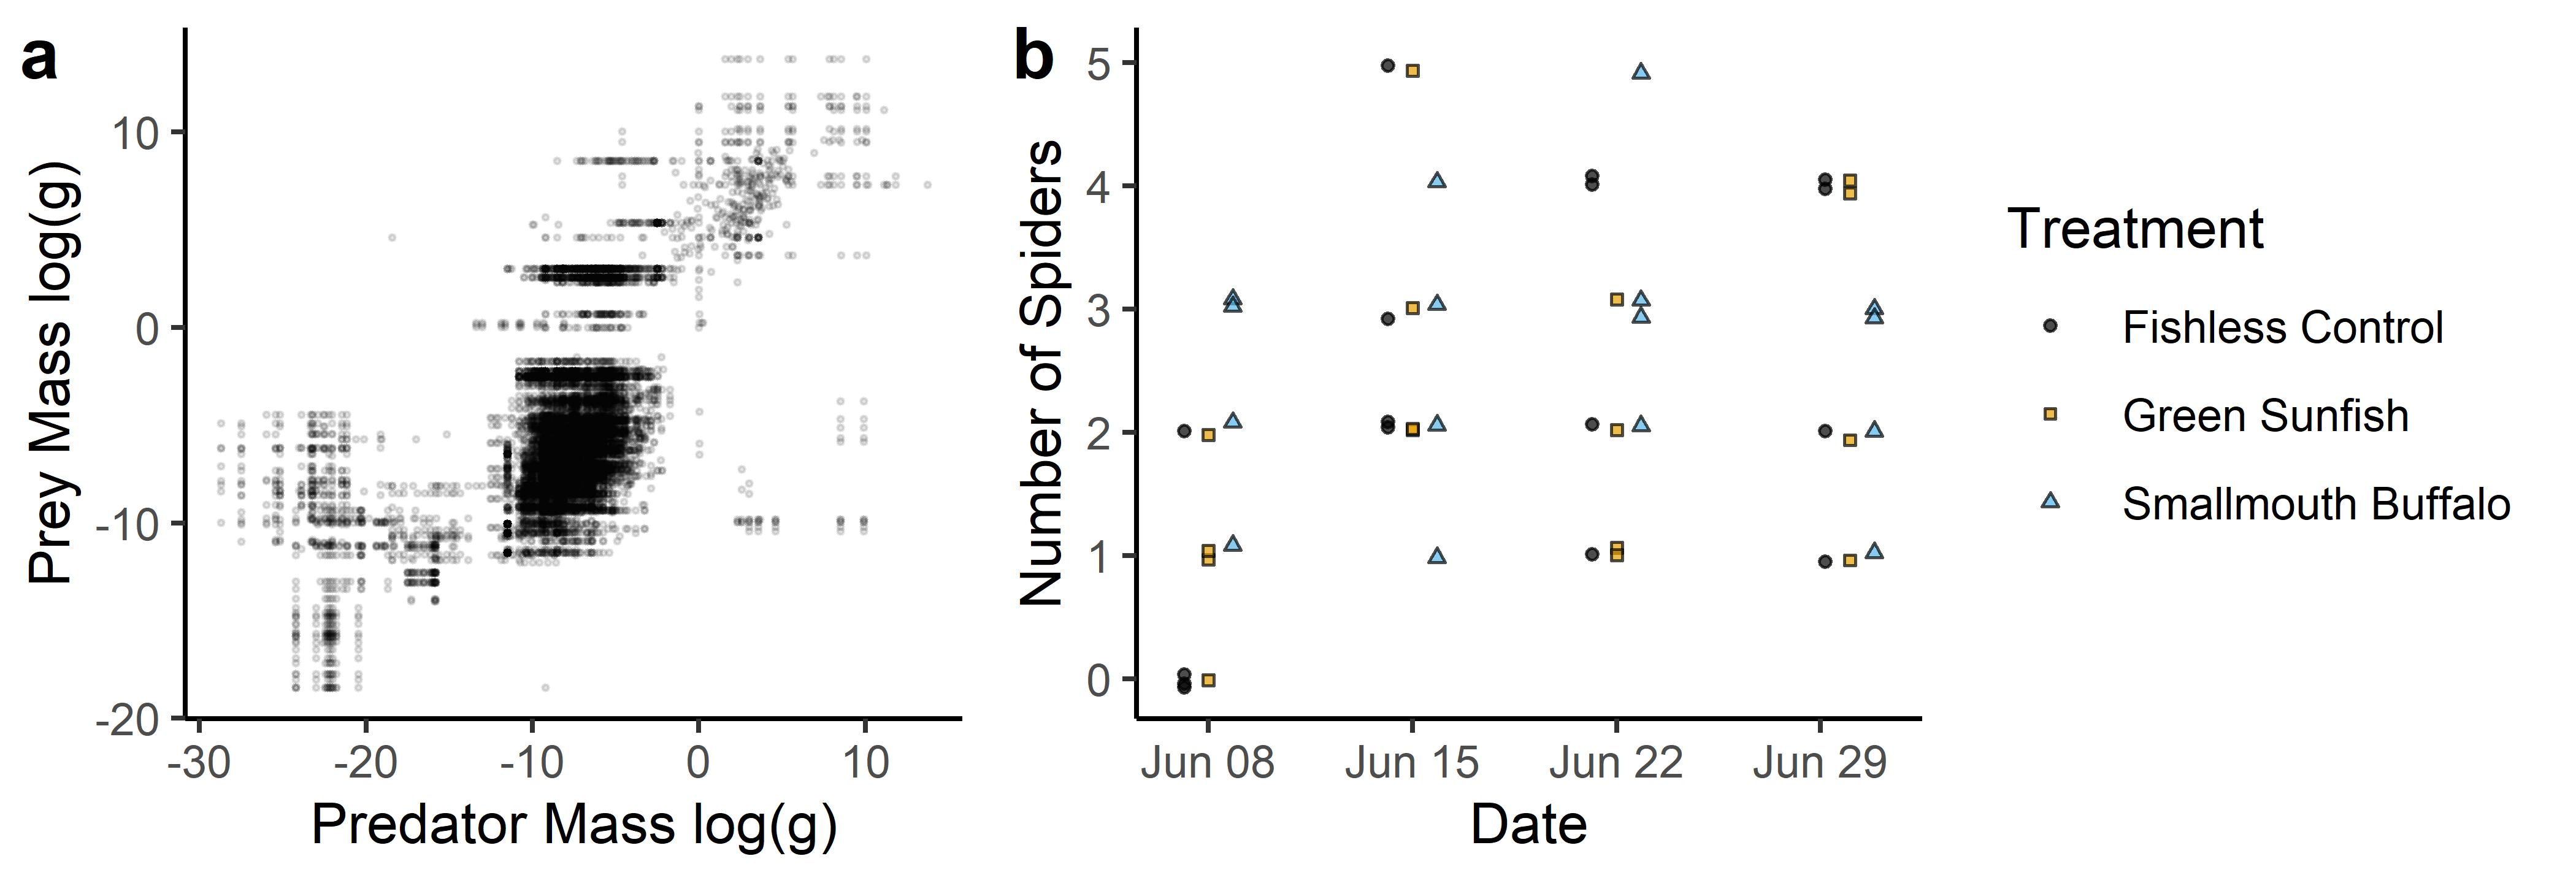
\includegraphics[width=1\linewidth]{C:/Users/Jeff.Wesner/Documents/GitHub/prior_predictive/plots/data_plots}

\newpage

\textbf{Figure 2}


\includegraphics[width=1\linewidth]{C:/Users/Jeff.Wesner/Documents/GitHub/prior_predictive/plots/mod_1}

\newpage

\textbf{Figure 3}


\includegraphics[width=1\linewidth]{C:/Users/Jeff.Wesner/Documents/GitHub/prior_predictive/plots/spiders_priors}

\newpage

\textbf{Supplementary Information}

Data and code are submitted as separate files. They are also available
here: \url{https://github.com/jswesner/prior_predictive}.


\includegraphics[width=41.67in]{C:/Users/Jeff.Wesner/Documents/GitHub/prior_predictive/plots/spider_supplementary}

Figure S1. The influence of the prior distributions on models estimating
spider density using data in Warmbold and Wesner (2018). Because of the
small sample size (n = 4 replicates), the prior specifications affect
the posterior. Compared to the weakest prior, the stronger prior is more
conservative, pulling each mean towards the prior mean. The strongest
prior (blue) is too strong, essentially swamping any information in the
data. Gray dots are raw data.

\end{document}
